\documentclass[conference]{IEEEtran}

\usepackage[canadian]{babel}
\usepackage{balance}
\usepackage{booktabs}
\usepackage{csquotes}
\usepackage{graphicx}
\usepackage{microtype}
\usepackage{tabularx}
\usepackage{tikz}
\usepackage{xcolor}
\usepackage{url}
\usepackage[hidelinks]{hyperref}
\usepackage{antonio-brand}
\usepackage[scaled=0.92]{inconsolata}
\usepackage[
  backend=biber,
  style=ieee,
  sorting=none,
  maxnames=6,
  minnames=1
]{biblatex}

\addbibresource{references.bib}
\usetikzlibrary{arrows.meta,positioning,calc}

% Antonio Sosa Brand System source:
% https://github.com/antonsoss/antonsoss-brand-system
% Commit: 8ce264b06b0f33591bfe5ccec92d3a0bfd889e47

\hypersetup{
  colorlinks=true,
  urlcolor=BrandLink,
  linkcolor=BrandLink,
  citecolor=BrandPrimary,
  pdftitle={Transaction Intelligence: Customer Segmentation and Behavioural Analytics},
  pdfauthor={Antonio Sosa},
  pdfsubject={MIA 5126 -- Essential Concepts in Data Science},
  pdfkeywords={banking analytics, customer segmentation, time-series forecasting, association rules, behavioural outliers}
}

\AtBeginBibliography{\footnotesize}
\setlength{\bibitemsep}{0.7pt}
\setlength{\bibhang}{0.8em}

\title{Transaction Intelligence: Customer Segmentation and Behavioural Analytics}

\author{
\IEEEauthorblockN{Antonio Sosa}
\IEEEauthorblockA{
MIA 5126 -- Essential Concepts in Data Science\\
Professor: Dr. Olubisi Runsewe\\
University of Ottawa, Ottawa, Canada
}
}

\begin{document}

\color{BrandText}
\maketitle

\begin{abstract}
This research-oriented applied project examines historical banking activity in the Czech Berka / PKDD'99 Financial Dataset. The objective is to identify interpretable account behaviour patterns while demonstrating relational data engineering, exploratory analysis, forecasting, association-rule mining, clustering, anomaly detection, and supervised learning without turning the work into a fraud or lending-decision system. Eight source tables were validated and transformed into account-level analytical data covering 4,500 accounts, 1,056,320 transactions, and 72 months. Monthly transaction counts were forecast with a chronological 12-month holdout; SARIMA achieved a mean absolute error of 2,321 transactions, compared with 3,858 and 3,942 for two naive baselines. K-means with five segments was selected using separation, inertia, stability, group size, and interpretability evidence; it obtained a silhouette score of 0.304 and a Davies-Bouldin score of 1.180. Sixteen accounts met a conservative two-method behavioural-outlier rule. The supervised loan case study was evaluated on 71 test loans that were not used during model training; logistic regression reached F1=0.545 and PR-AUC=0.471. The results support descriptive customer analysis and further investigation, not automated customer-treatment decisions.
\end{abstract}

\begin{IEEEkeywords}
banking analytics, customer segmentation, time-series forecasting, association rules, K-means, behavioural outliers, data engineering
\end{IEEEkeywords}

{\footnotesize
\noindent\BrandPrimaryText{\textbf{Project access:}}
The \href{https://transaction-intelligence-customer.onrender.com}{live application}
and \href{https://github.com/antonsoss/transaction-intelligence-customer-analytics}
{GitHub repository} provide the dashboard, API, notebooks, tests, and reproducible
artifacts used in this paper.
\par}

\section{Introduction}

Retail banking data are relational, temporal, and behaviourally varied. Accounts connect to customers, transactions, loans, cards, recurring orders, and regional context, so a useful analysis must preserve those relationships before reducing the data to one row per analytical unit. This project asks: \emph{Which account-level behaviour patterns emerge in the Berka data, how do they change over time, and how stable and interpretable are the resulting customer segments?} Supporting questions examine aggregate activity, service combinations, behavioural outliers, and whether a small loan-outcome exercise can demonstrate supervised methods without changing the project's descriptive centre.

The work is relevant to analysts seeking an evidence-based view of customer activity, service use, and changing portfolio coverage. It is deliberately bounded. Segment names summarize historical account patterns rather than fixed customer identities. Association rules are hypotheses, behavioural outliers are not fraud, and the loan case study is not a credit score. The scope is a reproducible local batch analysis plus a read-only Angular web dashboard. The project avoids causal claims and automated customer-treatment decisions.

\section{Background and Literature Review}

The Berka data originated in the PKDD'99 Discovery Challenge and describe an anonymized Czech bank through eight linked tables \cite{pkdd1999}. The Czech Technical University in Prague Relational Dataset Repository preserves accounts, clients, dispositions, transactions, standing orders, loans, cards, and districts, and explicitly warns that loan analysis must respect the loan-start cutoff \cite{ctufinancial}. Prior uses commonly emphasize loan outcomes; this project instead makes account behaviour and segmentation the primary contribution, with loan classification retained only as a limited course-method demonstration.

The analytical methods address complementary questions. Seasonal ARIMA models represent autocorrelation, differencing, and repeating seasonal structure in univariate series \cite{hyndman2008}. Apriori identifies frequent itemsets and derives association rules measured by support and confidence \cite{agrawal1994}; lift is used here to compare observed co-occurrence with an independence baseline. K-means partitions observations around centroids \cite{macqueen1967}, but no single internal measure proves a ``true'' number of clusters. Silhouette width evaluates cohesion and separation \cite{rousseeuw1987}, while the Davies-Bouldin index compares within-cluster scatter with between-cluster separation \cite{davies1979}. PCA reduces correlated variables into orthogonal components while retaining variance for interpretation and visualization \cite{jolliffe2016}. Isolation Forest provides a different, tree-based view of unusual observations \cite{liu2008}. The project combines these methods with stability, sensitivity, and plain-language profiling rather than selecting a model from one score alone.

\section{Methodology}

\subsection{Data Collection, Quality, and Architecture}

A reproducible database download and validation script exported the public MariaDB snapshot from the Czech Technical University in Prague Relational Dataset Repository, recording schemas, primary and foreign keys, row counts, and SHA-256 checksums. Source, exported, and local counts matched for all eight tables: 4,500 accounts, 5,369 clients and dispositions, 1,056,320 transactions, 6,471 orders, 682 loans, 892 cards, and 77 districts. Primary keys had no nulls or duplicates, and all eight foreign-key checks found zero orphaned rows. The two missing district attributes were retained as unavailable. No negative transaction amounts were found; 2,999 negative-balance records across 288 accounts were kept as valid financial states rather than automatically removed as errors.

Figure~\ref{fig:architecture} summarizes the batch medallion design. The Bronze layer preserves source CSV, DDL, provenance, and checksums. DuckDB \cite{raasveldt2019} reconstructs the relational schema and produces four Silver Parquet tables: clean transactions, account-client relationships, clean loans, and a 4,500-row account analytical base. Gold tables contain customer features, monthly activity, forecasts, service rules, segments, and anonymous dashboard outputs. Four executable notebooks own every transformation. A read-only FastAPI service exposes only eight selected aggregate or anonymous Parquet files; an Angular dashboard consumes the same typed endpoints. Neither layer retrains models or queries the external database at runtime.

\begin{figure*}[t]
\centering
\resizebox{\textwidth}{!}{%
\begin{tikzpicture}[
  node distance=0.38cm,
  box/.style={
    draw=BrandBorder,
    very thick,
    rounded corners=2pt,
    fill=BrandBackground,
    minimum height=0.78cm,
    text width=2.30cm,
    align=center,
    font=\scriptsize
  },
  source/.style={box, draw=BrandText},
  bronze/.style={box, draw=BrandMuted},
  silver/.style={box, draw=BrandPrimary},
  gold/.style={box, draw=BrandCode},
  runtime/.style={box, draw=BrandLink},
  presentation/.style={box, draw=BrandPrimary},
  arrow/.style={-{Latex[length=2mm]}, thick, draw=BrandMuted}
]
\node[source] (external) {External source\\CTU MariaDB};
\node[bronze, right=of external] (bronze) {Bronze: \texttt{data/raw}\\CSV, DDL, manifest, checksums};
\node[silver, right=of bronze] (silver) {Silver: \texttt{data/interim}\\DuckDB and clean Parquet};
\node[gold, right=of silver] (gold) {Gold: \texttt{data/processed}\\features, models, results};
\node[runtime, right=of gold] (api) {Read-only FastAPI\\curated endpoints};
\node[presentation, right=of api] (ui) {Angular dashboard\\five analytical views};
\coordinate (restmid) at ($(api.east)!0.5!(ui.west)$);
\node[rotate=90, font=\tiny, inner sep=0pt]
    at ($(restmid)+(0,3mm)$) {REST};
\draw[arrow] (external) -- (bronze);
\draw[arrow] (bronze) -- (silver);
\draw[arrow] (silver) -- (gold);
\draw[arrow] (gold) -- (api);
\draw[arrow] (api) -- (ui);
\end{tikzpicture}
}
\caption{Reproducible project architecture. Offline notebooks create validated artifacts; the deployed API and dashboard only present selected outputs.}
\label{fig:architecture}
\end{figure*}

\begin{table*}[t]
\caption{Notebook ownership and reproducible analytical outputs}
\label{tab:workflow}
\centering
\footnotesize
\begin{tabularx}{\textwidth}{p{0.235\textwidth} X X}
\toprule
\textbf{Notebook} & \textbf{Primary analytical work} & \textbf{Principal outputs} \\
\midrule
\nolinkurl{01_data_foundation_and_engineering.ipynb}
& Problem framing, relational validation, preparation policy, SQL joins, and local medallion architecture
& Four Silver tables: clean transactions, account-client relationships, clean loans, and the account analytical base \\
\nolinkurl{02_behavioral_and_temporal_analysis.ipynb}
& EDA, monthly aggregation, SARIMA forecasting, Apriori service associations, and account feature engineering
& Customer behaviour features, monthly activity, forecast results, and five filtered service rules \\
\nolinkurl{03_customer_segmentation.ipynb}
& Feature selection, Yeo-Johnson scaling, PCA, K-means/GMM comparison, stability tests, and consensus outliers
& Segment assignments and profiles, clustering evaluation, outlier cases, and saved preprocessing/PCA/K-means objects \\
\nolinkurl{04_validation_and_insights.ipynb}
& Leakage-aware loan demonstration, data-centric checks, error analysis, limitations, and final synthesis
& Model evaluation evidence plus anonymous, dashboard-ready tables and figures \\
\bottomrule
\end{tabularx}
\end{table*}

\subsection{EDA and Feature Construction}

Exploratory analysis covered transaction direction and operation, cash inflow and outflow, balances, loans, cards, standing orders, district context, and monthly activity. Because the number of observed accounts rose sharply, total activity was interpreted beside distinct active-account counts and average activity per active account. Thirty-nine account features were then created, including tenure, active-month ratio, transactions per observed month, average inflow and outflow, inflow-outflow ratio, balance level and volatility, negative-balance share, transaction diversity, and service indicators. A salary-like deposit flag used rule-based identification of recurring transfers and was treated as unverified. No customer-feature row was missing after construction.

\subsection{Evaluation Design and Reproducibility}

Temporal forecasting used the first 60 monthly observations for training and the final 12 months of 1998 for testing. Segmentation compared algorithms and values of $K$ without outcome labels. The supervised case used a fixed, stratified 70/30 split of completed loans, with imputation, scaling, and encoding fitted only on the 163 training loans. Every loan feature was available strictly before its loan date. Random state 42, saved preprocessing/PCA/clustering objects, artifact row-count assertions, Python and Angular tests, and versioned Docker deployment support reproducibility. Scikit-learn supplied the clustering, anomaly, and supervised estimators \cite{pedregosa2011}.

\section{Modelling}

\subsection{Temporal Forecast and Service Associations}

Monthly transaction counts were inspected using 12-month rolling statistics, additive decomposition, ACF/PACF, and augmented Dickey-Fuller tests. The displayed source transformations did not reject non-stationarity, so evaluation emphasized the chronological holdout. A declared SARIMA$(1,1,1)(1,1,0)_{12}$ model was compared with last-value and seasonal-naive forecasts using MAE and RMSE; 95\% forecast intervals represented model uncertainty.

For service analysis, each account became a binary basket containing yes/no service flags for card ownership, loans, standing orders, salary-like deposits, pensions, household payments, insurance payments, and leasing payments. Apriori searched itemsets of up to three services with support $\geq3\%$. Rules required confidence $\geq35\%$, lift $\geq1.05$, and one consequent. Structurally automatic standing-order rules were removed. The remaining rules were interpreted as questions for future validation, not personalized recommendations.

\subsection{Segmentation, PCA, and Behavioural Outliers}

Nine non-demographic features entered segmentation: monthly activity, average inflow, inflow-outflow ratio, average balance, negative-balance share, cash deposit and withdrawal shares, transaction diversity, and service diversity. Individual rare service flags, location, age proxies, tenure, and loan outcomes were excluded from distance calculations. Yeo-Johnson transformation reduced skew, followed by standard scaling. PCA was fitted for loadings and visualization rather than used to manufacture cluster evidence.

K-means models for $K=2,\ldots,8$ used 50 initializations. Full-covariance Gaussian mixtures with five initializations provided a soft-membership challenger over the same range. Selection considered inertia, silhouette, Davies-Bouldin, group sizes, five-seed adjusted Rand index (ARI) stability, preprocessing sensitivity, and business interpretability. Outlier review combined four signals: top 1\% within-segment centroid distance, bottom 1\% GMM membership, top 1\% robust within-segment deviation, and Isolation Forest with 1\% contamination. An account was retained only if at least two signals agreed.

\subsection{Completed-Loan Demonstration}

Only the 234 completed loans with known final outcomes were included: A means repaid without problems, and B means repaid with problems. Of these, 31 (13.25\%) recorded repayment problems. Inputs comprised amount, duration, statement frequency, and 11 account-activity measures calculated strictly before loan start. A prior-probability dummy, class-balanced logistic regression, class-balanced RBF SVM, and a class-balanced depth-3 decision tree were compared. Because the positive class was uncommon, precision, recall, F1, ROC-AUC, PR-AUC, and the confusion matrix were reported; PR evidence is especially informative under class imbalance \cite{saito2015}. This model estimates a historical two-outcome target used only for a limited supervised-learning case study and is not used by the segmenter.

\section{Performance Evaluation}

\subsection{Temporal and Association Findings}

The dataset covers January 1993 through December 1998. Active accounts increased from 96 to 4,424 and peaked at 4,483 in December 1997, so higher transaction totals partly reflect expanding coverage (Fig.~\ref{fig:temporal}). On the 1998 holdout, SARIMA obtained MAE 2,321 and RMSE 3,178 transactions. Last-value MAE/RMSE were 3,858/5,145; seasonal-naive values were 3,942/4,495. SARIMA therefore led the declared comparison, but one 12-month test window does not establish production reliability.

\begin{figure*}[t]
\centering
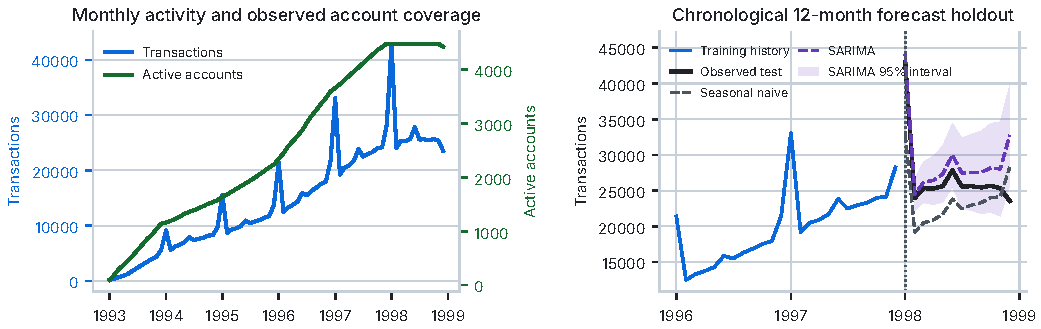
\includegraphics[width=\textwidth]{figures/temporal_analysis.pdf}
\caption{Left: monthly transaction totals and changing active-account coverage. Right: the declared 1998 holdout comparison with SARIMA uncertainty.}
\label{fig:temporal}
\end{figure*}

Five service rules survived filtering (Table~\ref{tab:rules}). The strongest was
\{\emph{household expenses, salary-like deposit}\}$\rightarrow$\{\emph{loan}\}, with support 3.07\%, confidence 54.55\%, and lift 3.60. It indicates that the combination occurred more often than expected under independence; it does not show cause, suitability, or customer interest. The three near-certain household-payment or standing-order consequents also require caution because they may reflect how recurring services were historically recorded rather than a useful recommendation opportunity.

\begin{table*}[t]
\caption{Filtered service-association hypotheses}
\label{tab:rules}
\centering
\footnotesize
\begin{tabularx}{\textwidth}{X X r r r}
\toprule
\textbf{Observed antecedent} & \textbf{Observed consequent} & \textbf{Support} & \textbf{Confidence} & \textbf{Lift} \\
\midrule
Household payment and salary-like deposit & Loan & 3.07\% & 54.55\% & 3.60 \\
Salary-like deposit & Loan & 4.67\% & 48.95\% & 3.23 \\
Pension deposit & Household payment & 16.44\% & 100.00\% & 1.31 \\
Insurance payment & Household payment & 11.84\% & 100.00\% & 1.31 \\
Pension deposit & Standing order & 16.36\% & 99.46\% & 1.19 \\
\bottomrule
\end{tabularx}
\begin{minipage}{0.98\textwidth}
\vspace{1pt}\scriptsize
\emph{Note:} ``Salary-like'' is a documented transaction-pattern heuristic, not a verified payroll label. Rules describe co-occurrence in this dataset and are not validated recommendations.
\end{minipage}
\end{table*}

\subsection{Segment Selection and Interpretation}

The first two principal components explained 63.4\% of variance; four explained 86.2\%. Figure~\ref{fig:clustering} shows that K-means at $K=5$ had the highest tested silhouette (0.304), the lowest tested Davies-Bouldin score (1.180), and a visible slowing of inertia improvement. Its smallest segment contained 251 accounts (5.58\%). The matched five-component GMM separated hard labels less clearly (silhouette 0.157; Davies-Bouldin 2.139), while its minimum BIC occurred at the search boundary $K=8$. K-means seed stability was high (mean ARI 0.996; minimum 0.995), although removing the power transform changed assignments substantially (ARI 0.469 and a two-account smallest group). This sensitivity is why the selected preprocessing is part of the saved model contract.

\begin{figure*}[t]
\centering
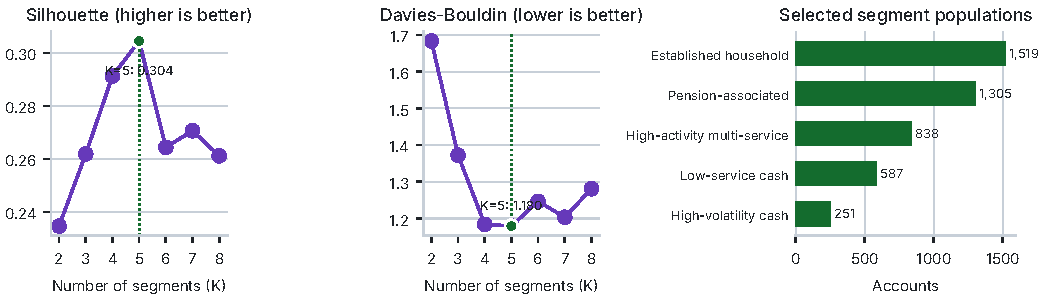
\includegraphics[width=\textwidth]{figures/clustering_analysis.pdf}
\caption{K-means selection evidence and the five account populations. Green markers identify the selected $K=5$ solution.}
\label{fig:clustering}
\end{figure*}

Table~\ref{tab:profiles} reports the profiles in original units. Names were assigned only after fitting from median activity, balance, channel, and service-use patterns. They summarize the observed accounts rather than define permanent customer types.

\begin{table*}[t]
\caption{Selected K-means segment profiles in original units}
\label{tab:profiles}
\centering
\scriptsize
\begin{tabularx}{\textwidth}{X r r r r X}
\toprule
\textbf{Segment} & \textbf{Accounts} & \textbf{Share} & \textbf{Median tx./month} & \textbf{Median avg. balance} & \textbf{Observed defining pattern} \\
\midrule
Established household users & 1,519 & 33.8\% & 5.54 & 45,623 & Larger inflows, mixed cash use, and common household payments and standing orders \\
Pension-associated households & 1,305 & 29.0\% & 4.90 & 20,900 & Lower recurring inflows, low cash-deposit share, and regular household payments \\
High-activity multi-service users & 838 & 18.6\% & 7.29 & 45,010 & Highest transaction and service diversity; cards, loans, and insurance are comparatively frequent \\
Low-service cash users & 587 & 13.0\% & 4.64 & 30,738 & Lower activity and diversity, a high cash-deposit share, and few observed services \\
High-volatility cash users & 251 & 5.6\% & 5.50 & 35,546 & Highest balance volatility, strongest negative-balance exposure, and high cash-withdrawal share \\
\bottomrule
\end{tabularx}
\begin{minipage}{0.98\textwidth}
\vspace{1pt}\scriptsize
\emph{Note:} Monetary values retain the dataset's source units. Profile labels are analyst summaries, not risk, value, age, or suitability labels.
\end{minipage}
\end{table*}

Sixteen accounts met the two-signal outlier rule; 15 had two agreeing signals and one had three. They are transparent review cases, not evidence of fraud or error.

\subsection{Supervised Results and Error Analysis}

Table~\ref{tab:loan} reports the 71-loan test results, which contained nine problem outcomes. Logistic regression provided the strongest balance of ranking and threshold measures: precision 0.462, recall 0.667, F1 0.545, ROC-AUC 0.892, and PR-AUC 0.471. Its confusion matrix contained 55 true negatives, seven false positives, three false negatives, and six true positives. The RBF SVM achieved slightly higher precision but lower recall and ranking performance; the shallow tree recovered more positives at the cost of many false alarms. The dummy model's PR-AUC of 0.127 approximated test prevalence.

\begin{table}[t]
\caption{Completed-loan test performance ($n=71$)}
\label{tab:loan}
\centering
\footnotesize
\begin{tabular}{lrrrrr}
\toprule
\textbf{Model} & \textbf{Prec.} & \textbf{Rec.} & \textbf{F1} & \textbf{ROC} & \textbf{PR} \\
\midrule
Dummy prior & 0.000 & 0.000 & 0.000 & 0.500 & 0.127 \\
Logistic regression & 0.462 & 0.667 & \textbf{0.545} & \textbf{0.892} & \textbf{0.471} \\
RBF SVM & \textbf{0.500} & 0.556 & 0.526 & 0.738 & 0.440 \\
Depth-3 tree & 0.259 & \textbf{0.778} & 0.389 & 0.723 & 0.245 \\
\bottomrule
\end{tabular}
\end{table}

Only pre-loan average outflow and inflow-outflow ratio had missing values (two each, 0.85\%); training-fitted median imputation handled them. Nevertheless, completed loans cover only 5.2\% of accounts and problem loans only 0.69\% of all accounts. Region-year subgroup counts and the single holdout are too small for strong generalization claims. Coefficients explain the fitted logistic model, but do not establish causal drivers of repayment.

\subsection{Data-Centric Validation}

Quality was evaluated as part of the analytical evidence rather than as a one-time cleaning step. Table~\ref{tab:audit} links the main checks to their effect on interpretation. The results distinguish invalid records from valid extreme values and behavioural outliers: negative balances were retained, while outlier flags were created only after segmentation and never treated as data errors.

\begin{table*}[t]
\caption{Data-centric validation summary}
\label{tab:audit}
\centering
\footnotesize
\renewcommand{\arraystretch}{0.96}
\begin{tabularx}{\textwidth}{p{0.15\textwidth} X X}
\toprule
\textbf{Check} & \textbf{Observed evidence} & \textbf{Analytical consequence} \\
\midrule
Relational integrity & Source, export, and local counts agreed; primary keys had no nulls or duplicates; eight foreign-key checks found no orphans & The joins and account-level base can be traced back to the source snapshot \\
Completeness & Two district attributes were unavailable; all 4,500 customer-feature rows were complete; two loan features each had 0.85\% missingness & District values remained missing; loan imputation was fitted on training data only \\
Temporal coverage & The history contains 72 months, while active accounts rose from 96 to 4,424 & Totals are interpreted beside account coverage, and forecasting uses a chronological holdout \\
Cluster robustness & Five-seed K-means ARI averaged 0.996, but removing the power transform produced ARI 0.469 & Random initialization was stable; preprocessing choice remained a material limitation \\
Supervised coverage & Only 234 completed loans and 31 problem outcomes were available; the test set contained nine positives & Results are a course-method demonstration, not evidence for customer-level lending decisions \\
Reproducibility & Four executable notebooks, saved model objects, row-count assertions, tests, and a versioned container connect analysis to presentation & Results can be rebuilt and traced, although reproducibility does not establish present-day validity \\
\bottomrule
\end{tabularx}
\end{table*}

\subsection{Strengths, Weaknesses, and Improvements}

Strengths include exact relational reconciliation, zero-orphan key validation, leakage-aware time cutoffs, explicit baselines, multiple cluster criteria, stability and preprocessing sensitivity checks, and traceable notebook-to-dashboard artifacts. The central weakness is external validity: one anonymized Czech bank from 1993--1998 cannot represent current customers, channels, regulation, or economic conditions. Account coverage changes across time; salary detection is heuristic; association rules do not establish causality; K-means works best when groups are compact and clearly separated; and internal cluster scores do not prove naturally existing groups. Forecasting has only 72 observations and one test year, while supervised conclusions rest on 31 positive loans.

Future evaluation should use rolling forecast origins, external or later banking data, formally labelled income categories, repeated loan validation, and customer-approved service-response data. Segment monitoring should compare profiles and assignment stability across time, and any operational use would require governance, privacy review, fairness testing, authentication, and human accountability.

\balance
\section{Summary and Conclusion}

The project demonstrates that the Berka relational data can be transformed into a reproducible account-level view without discarding source relationships or treating valid extremes as errors. Activity grew alongside observed account coverage; SARIMA reduced holdout error relative to two naive baselines; five filtered service associations supplied testable hypotheses; and a stable five-segment K-means solution summarized distinct activity, balance, channel, and service-use patterns. Sixteen consensus outliers identified unusual cases for explanation, not accusation. The small loan case showed that pre-loan information carried some historical signal, but its sample and coverage were too limited for lending decisions.

The main contribution is therefore not a predictive product. It is a traceable analytical workflow that connects data quality, time, segmentation, model evaluation, and responsible interpretation. The FastAPI and Angular application make selected results accessible, while the notebooks and saved artifacts remain the source of analytical truth.

\printbibliography[title={References}]

\end{document}
